\documentclass{article}
\usepackage[T2A]{fontenc}
\usepackage[utf8]{inputenc}
\usepackage[russian]{babel}
\usepackage{amsmath,amssymb,graphicx}
\begin{document}
\section{Лабораторная работа}
См. формулу \eqref{eq:two}, рисунок \ref{fig:plot}, таблицу \ref{tab:data} и источник \cite{book}.
\begin{equation}x=1\tag{1}\label{eq:one}\end{equation}
\begin{align}y&=2\tag{2}\label{eq:two}\\ z&=3\nonumber\\w&=4\end{align}
\begin{equation*}a=5\end{equation*}
\begin{figure}[h]
\centering
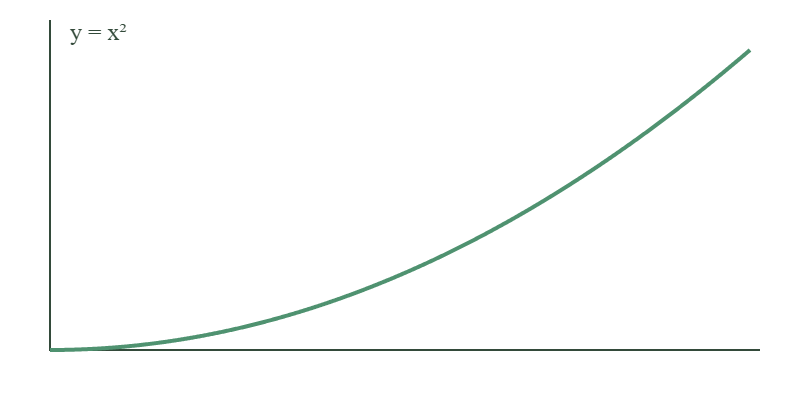
\includegraphics[width=0.8\linewidth]{plot.png}
\caption{Зависимость \(y=x^2\)}\label{fig:plot}
\end{figure}
\begin{table}[h]
\caption{Результаты}\label{tab:data}
\begin{tabular}{|c|p{4cm}|}
\hline
Номер & Измерение \\
1 & \(x=2\) \\
\multicolumn{2}{c}{Итого} \\
\hline
\end{tabular}
\end{table}
\begin{enumerate}
\item Подготовка\label{step:first}
\begin{itemize}
\item Датчик
\item Образец
\end{itemize}
\item Измерение
\begin{enumerate}\item Повторение\label{step:nested}\end{enumerate}
\end{enumerate}
Шаг \ref{step:first}, подпункт \ref{step:nested}.
\begin{thebibliography}{99}
\bibitem{book} Иванов. \textit{Физика}. 2025.
\end{thebibliography}
\end{document}
